This section describes building blocks that support efficient communication between work-items in a group. Some are fundamental building blocks that enable construction of custom algorithms, whereas others are higher level and describe common operations used by many kernels.\par

\hspace*{\fill} \par %插入空行
\textbf{Synchronization via Barriers}

The most fundamental building block for communication is the barrier function. The barrier function serves two key purposes:\par

First, the barrier function synchronizes execution of work-items in a group. By synchronizing execution, one work-item can ensure that another work-item has completed an operation before using the result of that operation. Alternatively, one work-item is given time to complete its operation before another work-item uses the result of the operation.\par

Second, the barrier function synchronizes how each work-item views the state of memory. This type of synchronization operation is known as enforcing memory consistency or fencing memory (more details in Chapter 19). Memory consistency is at least as important as synchronizing execution since it ensures that the results of memory operations performed before the barrier are visible to other work-items after the barrier. Without memory consistency, an operation in one work-item is like a tree falling in a forest, where the sound may or may not be heard by other work-items!\par

Figure 9-2 shows four work-items in a group that synchronize at a barrier function. Even though the execution time for each work-item may differ, no work-items can execute past the barrier until all work-items execute the barrier. After executing the barrier function, all work-items have a consistent view of memory.\par

\hspace*{\fill} \par %插入空行
Figure 9-2. Four work-items in a group synchronize at a barrier function
\begin{center}
	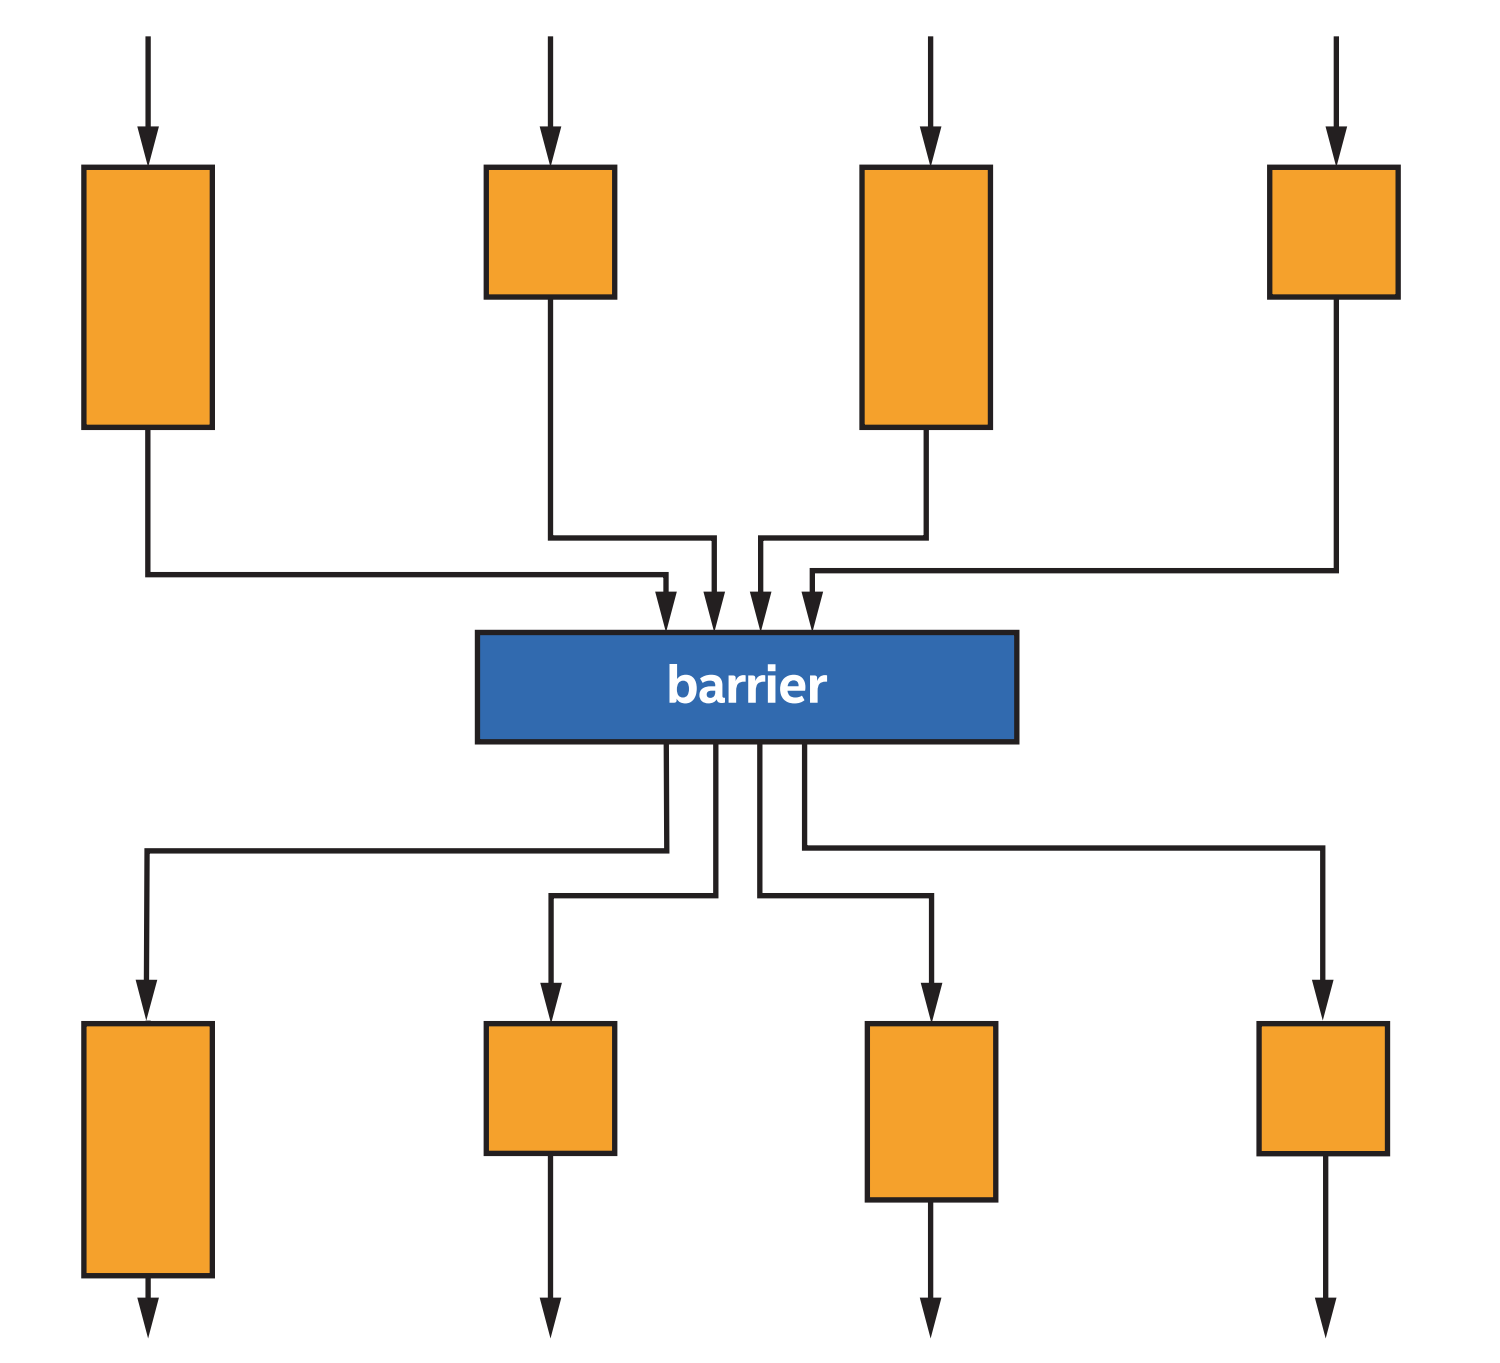
\includegraphics[width=1.\textwidth]{content/chapter-9/images/3}
\end{center}

\begin{tcolorbox}[colback=blue!5!white,colframe=blue!75!black, title=WHY ISN’T MEMORY CONSISTENT BY DEFAULT?]
For many programmers, the idea of memory consistency—and that different work-items can have different views of memory—can feel very strange. Wouldn’t it be easier if all memory was consistent for all work-items by default? The short answer is that it would, but it would also be very expensive to implement. By allowing work-items to have inconsistent views of memory and only requiring memory consistency at defined points during program execution, accelerator hardware may be cheaper, may perform better, or both.
\end{tcolorbox}

Because barrier functions synchronize execution, it is critically important that either all work-items in the group execute the barrier or no work-items in the group execute the barrier. If some work-items in the group branch around any barrier function, the other work-items in the group may wait at the barrier forever—or at least until the user gives up and terminates the program!\par

\begin{tcolorbox}[colback=blue!5!white,colframe=blue!75!black, title=COLLECTIVE FUNCTIONS]
When a function is required to be executed by all work-items in a group, it may be called a collective function, since the operation is performed by the group and not by individual work-items in the group. Barrier functions are not the only collective functions available in SYCL. Other collective functions are described later in this chapter.
\end{tcolorbox}

\hspace*{\fill} \par %插入空行
\textbf{Work-Group Local Memory}

The work-group barrier function is sufficient to coordinate communication among work-items in a work-group, but the communication itself must occur through memory. Communication may occur through either USM or buffers, but this can be inconvenient and inefficient: it requires a dedicated allocation for communication and requires partitioning the allocation among work-groups.\par

To simplify kernel development and accelerate communication between work-items in a work-group, SYCL defines a special local memory space specifically for communication between work-items in a work-group.\par

\hspace*{\fill} \par %插入空行
Figure 9-3. Each work-group may access all global memory, but only its own local memory
\begin{center}
	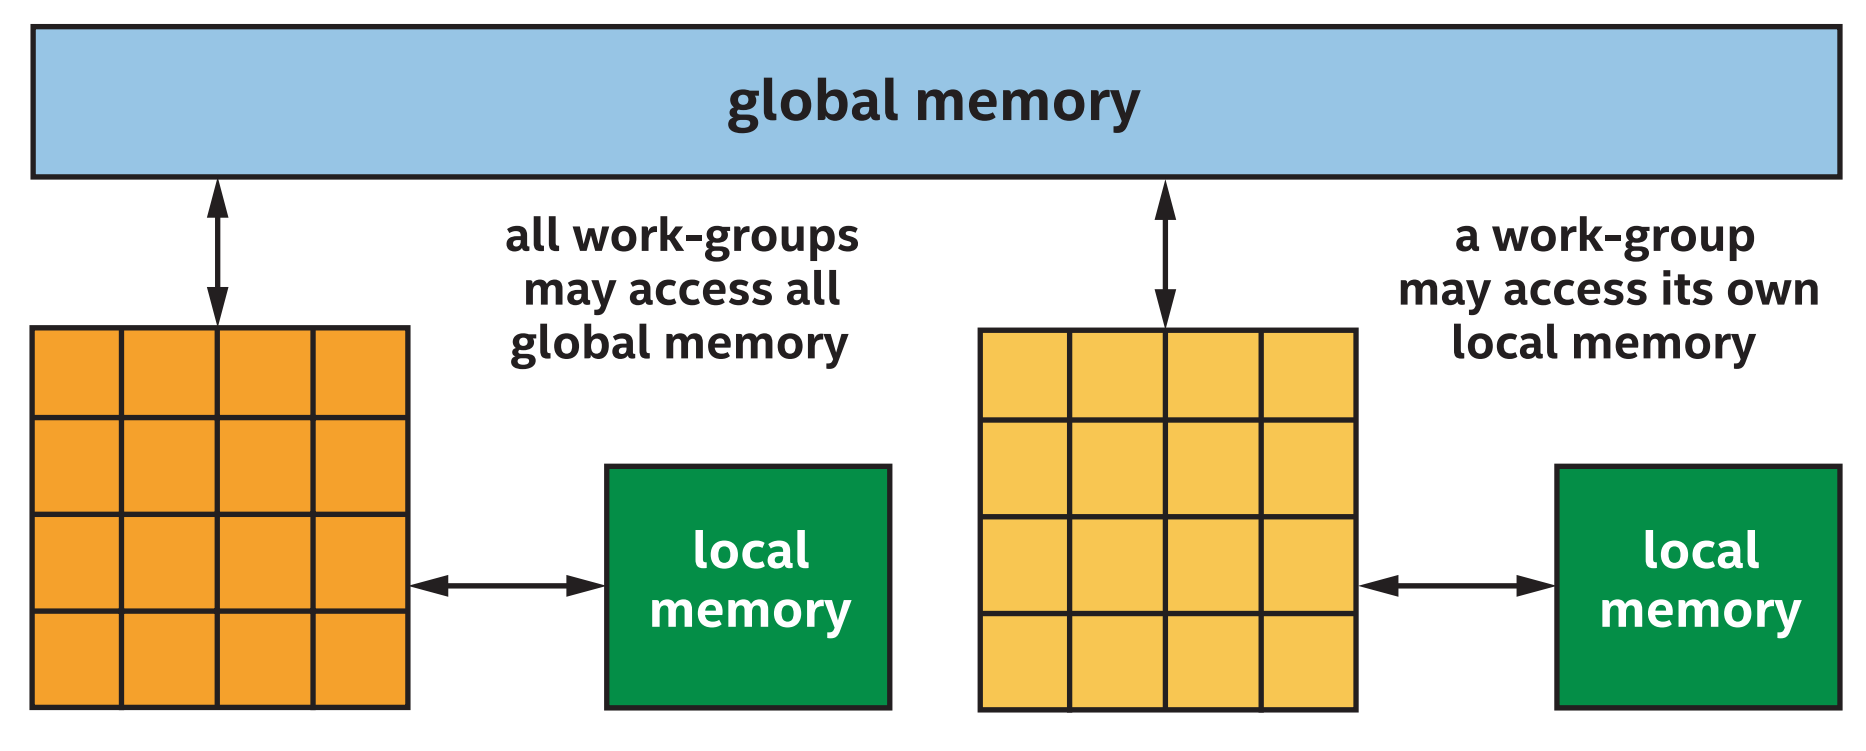
\includegraphics[width=1.\textwidth]{content/chapter-9/images/4}
\end{center}

In Figure 9-3, two work-groups are shown. Both work-groups may access USM and buffers in the global memory space. Each work-group may access variables in its own local memory space, but cannot access variables in another work-group’s local memory.\par

When a work-group begins, the contents of its local memory are uninitialized, and local memory does not persist after a work-group finishes executing. Because of these properties, local memory may only be used for temporary storage while a work-group is executing.\par

For some devices, such as for many CPU devices, local memory is a software abstraction and is implemented using the same memory subsystems as global memory. On these devices, using local memory is primarily a convenience mechanism for communication. Some compilers may use the memory space information for compiler optimizations, but otherwise using local memory for communication will not fundamentally perform better than communication via global memory on these devices.\par

For other devices though, such as many GPU devices, there are dedicated resources for local memory, and on these devices, communicating via local memory will perform better than communicating via global memory.\par

\begin{tcolorbox}[colback=red!5!white,colframe=red!75!black]
Communication between work-items in a work-group can be more convenient and faster when using local memory!
\end{tcolorbox}

We can use the device query info::device::local\_mem\_type to determine whether an accelerator has dedicated resources for local memory or whether local memory is implemented as a software abstraction of global memory. Please refer to Chapter 12 for more information about querying properties of a device and to Chapters 15, 16, and 17 for more information about how local memory is typically implemented for CPUs, GPUs, and FPGAs.\par





































